\section{Metric, Tokenization, and Decoder Details}
\label{app:metric}
The AutoVLA GT trajectory contains ten future poses in the local current-ego frame ($x$ forward, $y$ left, heading in radians), at 0.5\,s spacing. GT tokenization greedily evaluates all 2,048 codebook motions at each step. Each motion is represented by the four corners of a $2.0\times4.8$\,m vehicle box at its final substep. The selected token minimizes the sum of corner distances to the GT box; tokenization advances from the selected token's pose, not the exact GT pose. Decoding chains codebook motions from the origin. Thus, token identity, local displacement, decoded endpoint, and GT error are distinct quantities.

The coarse acceptance label uses only the A rule from the existing P/R/A evaluation. P and R labels do not define the failure stratum. Longitudinal semantics use the mean speeds of the first two and last two steps. STOP requires total distance below 1\,m and final speed below 0.5\,m/s. Below 0.5\,m/s, an absolute speed change above 0.8\,m/s is used; otherwise ratios of 1.25 and 0.75 distinguish acceleration and deceleration. Lateral semantics use final lateral displacement beyond 2\,m or final-step heading beyond $15^\circ$. Predicted longitudinal semantics must belong to the GT class set obtained by shifting GT final speed over an 11-point tolerance grid of $\pm\max(0.5,0.15\max(v))$\,m/s. Lateral acceptance uses a $5\times5$ grid spanning $\pm1$\,m lateral displacement and $\pm10^\circ$ heading. A plan is accepted only when both axes pass. These fixed thresholds were originally documented for a shorter horizon and are applied here to the ten-step plan; the severe event is an operational surrogate, not a standard driving safety endpoint.

Development units include the original token and distance-matched alternatives at $t^*$. Alternatives are selected across eight directional sectors, with a 5\,mm minimum distance tolerance and relative tolerances widened only according to the stored rule. The same GT projection and acceptance code are retained in P1-C. Scene selection uses the natural plan before the interventions, rather than selecting on a treated outcome.

The shared cached prefix comprises the prompt, stored planning stub, and actions before $t^*$. The span beginning with the forced token is re-encoded after each edit; the cache is cropped back to the shared prefix. Common-random-number keys depend on scene, perturbation, and generation position, with seed zero and temperature 0.01. Matched-prefix cells are decoded separately at batch size one from a common prefix. Their natural/no-op cells reproduce the source bank; P1-C also reproduces all 2,160 stored Normal rows used in that comparison. These checks do not imply exact invariance to all batch shapes or attention backends.

\section{Estimation, Interval Policy, and Coverage Checks}
\label{app:stats}
For paired unit differences $d_{su}$ in scene $s$, define $d_s=|U_s|^{-1}\sum_u d_{su}$. With fixed scene weights $w_s$, the estimator and cluster totals are
\begin{equation}
\widehat\theta=\frac{\sum_g N_g}{\sum_g D_g},\qquad
N_g=\sum_{s\in g}w_s d_s,\qquad D_g=\sum_{s\in g}w_s.
\end{equation}
Failure-stratum weights are one; evaluation-frame weights are inverse inclusion probabilities. The zero-null sign-flip statistic compares $|\sum_gN_g|$ against all sign changes of $N_g$. The assumed independent, sign-symmetric totals concern the chosen cluster axis. A few large clusters or shared days/vehicles are substantive limitations, not repaired by exact enumeration. Holm adjustment controls its family error only if the individual tests' assumptions hold.

The approximate cluster-$t$ interval uses
\begin{equation}
\widehat{\mathrm{se}}(\widehat\theta)=
\frac{\sqrt{\frac{G}{G-1}\sum_g(N_g-\widehat\theta D_g)^2}}{\sum_gD_g},
\qquad \widehat\theta\ \pm\ t_{G-1,1-\alpha/2}\widehat{\mathrm{se}}.
\end{equation}
The interval is an approximate precision summary. It is not obtained by inverting a shifted binary sign-flip test; that procedure can violate symmetry in the presence of ties and has been withdrawn. No binary sign-flip-inversion interval or shifted sign-flip equivalence conclusion is used in this revision.

\begin{table}[ht]
\centering\small
\caption{Post-hoc contrast-specific simulation checks. Each contrast has 16 planned scenarios and 5,000 replicates per scenario. The entries are ranges of coverage across those scenarios, not coverage estimates for the actual research result. MC upper limits refer to Wilson 95\% limits at each minimum.}
\label{tab:coverage}
\begin{tabular}{@{}lrrrr@{}}\toprule
Contrast & Units / scenes / drives & Nominal 95\% coverage & MC upper at minimum & Nominal 90\% coverage\\\midrule
Development RN & 365 / 52 / 13 & 92.8--99.1\% & 93.5\% & 87.5--97.6\%\\
P1-C F RN & 748 / 105 / 18 & 92.9--97.2\% & 93.6\% & 87.6--93.6\%\\
P1-C F RV & 748 / 105 / 18 & 92.8--98.8\% & 93.5\% & 87.7--97.2\%\\
Matched-prefix F $C_{\NAT}$ & 711 / 100 / 18 & 93.1--97.7\% & 93.7\% & 87.5--94.8\%\\\bottomrule
\end{tabular}
\end{table}

The October 19 sensitivity plan was written before those computations, but after the research effects and earlier interval study had been seen. Its first model retains each scene's observed discordance in the paired differences, then varies their mean; its second independently generates treatment and reference arms from the observed reference-arm rate and an imposed shift. The first is a model of differences and does not preserve every observed reference marginal under all shifts. Both use the real scene sizes and drive membership. Target effects include zero, both signs of 10\,pp, and the observed effect scale; drive heterogeneity is 0 or 5\,pp. Clipping means some target shifts cannot be reached. Coverage is assessed against each replicate's realized conditional truth, not the unclipped target.

The first fixed-scene checks fall to approximately 93\% coverage near the null (Table~\ref{tab:coverage}); empirical-cell alternatives condition on the observed scenes. These checks alone do not validate a population of newly sampled drives. Development RV and direction/magnitude, and matched-prefix $C_{\GT}$/$C_{\mathrm{src}}$, lack direct contrast-specific coverage checks. Their intervals remain approximate summaries by structural analogy.

\subsection{Additional finite-frame and new-drive audit}
The supplied follow-up distinguishes two simulation designs. D3 fixes a pseudo-population for the eligible frame and resamples accepted scenes within logs using the actual sampling design and weights. Unsampled outcomes are imputed by cycling sampled scenes within each log. D2 additionally resamples drives with replacement, with accepted-scene resampling and outcome variation. Its support is limited to the 18--24 observed drive structures; it does not establish arbitrary new-drive coverage or include day/vehicle dependence.

Joint four-cell label swaps preserve within-unit pairing for the factorial interaction before scene and drive aggregation. The plan considers four effect levels (zero, both signs of half the observed effect, and observed), two couplings, and 5,000 cluster-$t$ replicates per scenario (1,000 for the bootstrap comparator). It was fixed before these simulations, after the original research effects had been observed; this is a post-hoc assessment. Coverage is evaluated against the generated truth, not an unclipped requested shift.

\begin{table}[ht]
\centering\small
\caption{New post-hoc nominal-95\% cluster-$t$ coverage ranges. D3 is the finite eligible frame; D2 resamples drives. F is a census, so D3 is not run for F contrasts. These ranges describe the checked data-generating scenarios, not guarantees for the research results.}
\label{tab:coverage_new}
\begin{tabular}{@{}lrrl@{}}\toprule
Contrast & D3 coverage, \% & D2 coverage, \% & Display policy\\\midrule
E RN & 93.7--100.0 & 90.8--94.0 & Approximate eligible-frame interval\\
E RV & 95.3--99.5 & 88.6--96.0 & Point only in this revision\\
E4 $C_{\NAT}$ & 94.0--99.5 & 89.0--94.7 & Point only in this revision\\
E4 $C_{\GT}$ & 93.0--100.0 & 92.7--93.8 & Approximate eligible-frame interval\\
E4 $I$ & 92.8--99.4 & 91.2--93.1 & Approximate eligible-frame interval\\
F RN & -- & 91.5--93.7 & Approximate\\
F $C_{\NAT}$ & -- & 93.6--94.3 & Approximate overall\\
F $I$ & -- & 88.6--93.7 & Interval withheld\\\bottomrule
\end{tabular}
\end{table}

The finite-frame E RV and E4 $C_{\NAT}$ intervals could be shown only with that narrow interpretation under the supplied policy; we conservatively retain points for these rows throughout the displayed comparison. F's interaction interval is withdrawn. E4's interaction retains an approximate interval under the joint-cell check, with no equivalence margin and no inference of equality. The bootstrap comparator generally undercovers more. No effect estimate or zero-null $p$ value changes. Withholding an interval does not certify the independence/symmetry assumptions of its sign-flip test.

\begin{table}[ht]
\centering\small
\caption{Repeated contrasts and updated frame-interval status (pp). Brackets are approximate nominal-95\% drive-cluster $t$ intervals; they are not coverage-validated bounds. Holm families include direction/magnitude ($\alpha=0.05$ in F; 0.025 in E). A dash is a withheld interval.}
\label{tab:repeated_full}
\begin{tabular}{@{}llrrr@{}}\toprule
Cohort & Contrast & Estimate & Approximate interval & Holm $p$\\\midrule
Development F & RN & $-39.8$ & $[-50.9,-28.7]$ & $7.3\times10^{-4}$\\
 & RV & $+28.6$ & $[20.1,37.2]$ & $7.3\times10^{-4}$\\
P1-C F & RN & $-34.2$ & $[-39.0,-29.4]$ & $2.3\times10^{-5}$\\
 & RV & $+26.8$ & $[22.1,31.5]$ & $6.1\times10^{-5}$\\
P1-C E & RN & $-4.1$ & $[-6.2,-2.0]$ (frame) & $1.1\times10^{-5}$\\
 & RV & $+3.6$ & -- & $2.9\times10^{-6}$\\\bottomrule
\end{tabular}
\end{table}

Additional E4 frame intervals are $[0.9,5.8]$\,pp for $C_{\GT}=3.3$\,pp and $[-2.2,0.9]$\,pp for $I=-0.7$\,pp. E4 $C_{\mathrm{src}}$, E direction/magnitude, higher-level cluster axes, and small subsets have no retained primary interval. Earlier numerical cutoffs used to choose interval methods are historical selection rules, not nominal-coverage guarantees. We do not infer that no interval procedure could work.

The motion-control intervals are drive percentile bootstraps (10,000 draws), retained only as descriptive uncertainty. The window-recovery interval is a joint numerator/denominator bootstrap and likewise has unchecked coverage. Neither was validated by the binary-contrast simulations. Margin checks based on approximate 90\% $t$ intervals are sensitivity analyses and do not supply confirmatory guarantees.

\section{Matched-Prefix Domains and Higher-Level Clusters}
\label{app:matched}
The E4 domain uses $t^*\leq4$ and at least three generated suffix positions under the primary anchor. Its 1,775 eligible scenes comprise 100 F and 1,675 accepted scenes; all F scenes and 212 accepted scenes are analyzed. This differs from the repeated-schedule E domain ($t^*\leq7$; 105 F scenes plus 248 sampled accepted scenes). We do not apply E weights to E4 or describe either as an unconditioned driving population.

The primary older factor has exactly one position ($t^*+1$). A secondary anchor at $a=t^*+4$ changes two older positions and the remaining horizon. It is a different comparison. A secondary interaction in the weighted frame was $+2.7$\,pp with unadjusted $p=0.0046$, reinforcing that the primary near-zero interaction does not establish general context independence. All edits remain present in later contexts; no true release is tested.

\begin{table}[ht]
\centering\small
\caption{Primary matched-prefix F tests by cluster axis. Entries are raw $p$ / Holm $p$. Day--vehicle clustering does not allow arbitrary sharing of days or vehicles across groups; connected components address that more conservative grouping.}
\label{tab:cluster}
\begin{tabular}{@{}lrrr@{}}\toprule
Contrast & Drive (18 groups) & Day--vehicle (10 groups) & Connected component (6 groups)\\\midrule
$C_{\GT}$ & $0.0000153/0.0000458$ & $0.00195/0.00781$ & $0.03125/0.125$\\
$C_{\NAT}$ & $0.00000763/0.0000305$ & $0.00195/0.00781$ & $0.03125/0.125$\\
$I$ & $0.920/0.920$ & $0.848/0.848$ & $0.750/0.750$\\
$C_{\mathrm{src}}$ & $0.000732/0.00146$ & $0.00977/0.0195$ & $0.0625/0.125$\\\bottomrule
\end{tabular}
\end{table}

The component graph is constructed on all 312 sampled E4 scenes and then held fixed across strata. Components can contain multiple days and vehicles linked by reuse. Ten day--vehicle combinations are shared between development and P1-C, and two P1-C components merge when development is added. Thus, neither rerunning the existing P1-C drives nor regrouping them creates independent external validation. For $C_{\mathrm{src}}$, one component has the opposite sign; it does not attain the raw minimum of 0.03125 reached by the other two F contrasts.

\section{Motion Controls and Computation Settings}
\label{app:motion}
The primary numerical check uses P1-A family G: 1,453 units, with 364 in F and 1,089 in the selected accepted stratum. Each unit retains its own sector perturbation, frozen reference, seed, and original batch of ten rows. There are 14,530 rows per setting and 43,590 total. Source-token equality is exact for all S0 rows. The executed prefix is locked throughout; context-edited tokens are not substituted into that prefix.

CM repeats a local body-frame motion including heading change; it is not zero-turn constant velocity. CV0 removes turning. CTRV-K3 estimates constant turn rate and velocity from three prefix steps; CTRA-2 includes acceleration. The learned prefix control is a motion MLP trained on 145 drives with 26 validation drives, averaged across three seeds. Its prefix-plus-ego variant is secondary. These controls compare response under the same injected motion change; they neither isolate an autoregressive architectural effect nor match pretraining data or capacity.

\begin{table}[ht]
\centering\small
\caption{F endpoint-response excess (m) in the numerical follow-up. Brackets are descriptive drive-bootstrap intervals with unchecked coverage. Holm columns belong to one 12-test SE/SF family; S0 is a reference, not another member of that family.}
\label{tab:numeric}
\begin{tabular}{@{}lrrrrr@{}}\toprule
Control & S0 & SE [interval] & SE Holm $p$ & SF [interval] & SF Holm $p$\\\midrule
Coordinate accumulation & 4.37 & 4.06 [3.35,4.65] & 0.0029 & 4.45 [3.63,5.00] & 0.0029\\
CM & 2.35 & 2.04 [1.37,2.55] & 0.0029 & 2.43 [1.62,2.99] & 0.0029\\
CV0 & 4.02 & 3.71 [2.92,4.32] & 0.0029 & 4.10 [3.20,4.68] & 0.0029\\
CTRV-K3 & 3.02 & 2.71 [1.92,3.26] & 0.0029 & 3.10 [2.19,3.71] & 0.0029\\
CTRA-2 & 1.43 & 1.12 [0.57,1.76] & 0.0088 & 1.51 [0.84,2.08] & 0.0088\\
Learned prefix & 1.97 & 1.65 [1.00,2.44] & 0.0088 & 2.04 [1.32,2.73] & 0.0059\\\bottomrule
\end{tabular}
\end{table}

SE and SF change some sampled suffixes despite identical seed keys. Approximate row-level endpoint shifts average 0.34 and 0.33\,m. The F excess changes by the same amount for every baseline because baseline responses are frozen. A pre-fixed descriptive materiality threshold was not crossed, but the broad paired intervals preclude claiming numerical equivalence. E-family, GF1/GF3, and near-zero self-reference FDE rows were not included. The original $+4.37$\,m geometry result has several analysis rows with different endpoints, seeds, and multiplicity families; Table~\ref{tab:numeric} consistently uses the B\_NUMERIC response definition in the endpoint-response equation in the main paper.

\section{Retained Windows, Transient Exposure, and Secondary Contrasts}
\label{app:window}
The restored R9 window experiment replaces three fixed positions with GT and retains them in every later context. Its scene-weighted severe-event levels are 45.12\% (Normal), 7.57\% (three-position window), and 3.43\% (Full-GT). The recovered fraction is
\begin{equation}
\frac{45.12-7.57}{45.12-3.43}=90.1\%.
\end{equation}
The numerator is 37.5\,pp and denominator 41.7\,pp. The descriptive ratio-bootstrap interval is $[81.2,98.9]\%$ over 365 units, 52 scenes, and 13 drives. Units average 2.96 GT positions and 1.90 effective token changes. This is a fraction of an oracle correction effect, not 90\% task success, a lower bound of 90\%, or a demonstration of persistent recovery after removing GT. The mean 3.8 steps after the last added GT position still read the retained GT positions.

A post-hoc alternative shows each of three corrected tokens only once as the latest context, then restores its own generated value in later contexts. Recovery is 78.3\% with descriptive interval $[64.0,86.6]$ (326 units, 46 scenes, 12 drives). This is a transient-exposure comparison, not a persistent-window-then-release experiment with matched exposure. Under a fixed ten-token horizon, matching absolute intervention position and subsequent horizon simultaneously is structurally limited.

P1-B does not establish an early-position advantage. Its three-position early/late contrast satisfies a $\pm10$\,pp margin only under the approximate interval sensitivity analysis; this does not establish positional equality in general. Direction-minus-magnitude is $+9.9$\,pp in development (approximate interval $[0.9,18.8]$), but $+6.2$\,pp in P1-C F (sensitivity interval $[-0.1,12.4]$, primary $p=0.073$). Direction superiority is not replicated. A nearby-GT alternative yields only an exploratory margin result under revised intervals; it does not establish that token identity is irrelevant or that nearby tokens are as effective as GT.

\section{SpatialVLA Task-Specific Success and State Reuse}
\label{app:spatial}
Success differences use paired outcomes with initial-state clustering within task, and equal task weights for pooled means. For independent paired states the corrected interval is Newcombe method 10; repeated states use a Rao--Scott-style design-effect adjustment, and task means are combined using MOVER. Margin tests are obtained from the corrected paired procedures, not shifted binary sign-flip inversion. These are post-hoc approximate corrections with limited simulation support, not universal exact guarantees. The 10\,pp margin was original; 5\,pp is a post-hoc sensitivity margin, and neither is a field-wide default.

\begin{table}[ht]
\centering\small
\caption{P1-D success by task under physical-state clustering (pp). These corrected approximate 95\% intervals show why pooled bounds do not establish per-task bounds. No $\pm5$\,pp task or pooled equivalence survives the reported multiplicity correction.}
\label{tab:spatialtasks}
\begin{tabular}{@{}lllrr@{}}\toprule
Setting & Contrast & Task (physical states) & Estimate & Approx. interval\\\midrule
r1e4 & $R-N$ & coke (120) & 0.0 & $[-6.5,6.5]$\\
 & & move\_near (10) & $+1.7$ & $[-8.4,11.7]$\\
 & $C-F$ & coke (120) & $+4.2$ & $[-2.8,11.3]$\\
 & & move\_near (10) & $+0.8$ & $[-6.9,8.6]$\\
r4e1 & $R-N$ & coke (120) & $+1.7$ & $[-8.3,11.6]$\\
 & & move\_near (10) & $+0.8$ & $[-8.4,10.0]$\\
 & $C-F$ & coke (120) & $-4.2$ & $[-14.0,5.8]$\\
 & & move\_near (10) & $+4.2$ & $[-8.6,16.7]$\\\bottomrule
\end{tabular}
\end{table}

For the four pooled direct contrasts in the success panel in the main paper, Holm-adjusted $\pm10$\,pp equivalence $p$ values under physical clustering are 0.00668, 0.00862, 0.01077, and 0.01077, respectively. The corresponding $\pm5$\,pp values are 0.338, 0.344, 0.344, and 0.344. These quantify the stated margin under the corrected approximate method; a nonsignificant zero-effect test alone would not establish equivalence~\citep{lakens2017equivalence}.

Earlier experiments 34/35 reuse the same ten \texttt{move\_near} layouts. Experiment 34 lacks actual TCP records and object initial-state logs; cumulative commanded motion must not be called measured TCP displacement. Object reset drift of up to 0.26\,mm was observed, and complete paired state restoration was not verified for these runs. The supplied P1-D episode audit records restore\_ok for all 3,840 branch episodes; the 960 natural roots have no restoration field. This verifies the recorded check, not a full-state hash audit of every controller/ensemble variable. The earlier experiment-35 $R-N=-6.2$\,pp result becomes uncertain under clustering and is not replicated in P1-D. It is excluded from the core success evidence.

Direct effects and execution-setting interactions are separate families. Corrected success-interaction equivalence is not universal across every reported comparison; for example, the pooled physical r2e1-minus-r1e1 $C-F$ interaction has adjusted margin $p=0.051$. We do not retain the older blanket claim that every interaction satisfies the 10\,pp margin. The trajectory-area execution comparisons in the main text use their original continuous-metric descriptive intervals.

\section{Descriptive Results in Other Models}
\label{app:othermodels}
Impromptu VLA generates coordinate text rather than motion codes. Earlier analyses show large correction and reinsertion contrasts across 20 drives, but intervention-path parity was not established. Identical paths and batches reproduce bitwise; changing batch composition or splitting prefill/decoding changes some outputs. Condition-correlated batching has not been ruled out. The Reverse condition also uses the intervention branch's own prior waypoint, unlike AutoVLA's separate Normal source. We retain these as descriptive observations, not strong cross-model replication or independent architectural evidence.

OpenVLA generates dimensions autoregressively within one control step and does not explicitly reuse its preceding step's action tokens in the next call. Its experiment covers ten LIBERO-Spatial tasks and ten states per task. The reported 92.6\% token response counts cases with at least one later dimension shifting by at least the injected effective bin count. It is not a failure rate, a physical-motion amplification rate, or a temporal action-prefix replication. Corrected success $C-F$ is $-3$\,pp with a Newcombe interval of $[-11.9,5.9]$ at eight bins, without established equivalence. Unperturbed reruns themselves disagree on 20\% of episode outcomes. The intervention-path gate remains unrun, so this model is excluded from the principal mechanistic evidence. We do not use 20\% as a proven noise floor or conclude that any smaller intervention effect is absent.

\section{Provenance, Reproduction, and Remaining Limits}
\label{app:provenance}
The experimental record separates exploratory discovery, planned follow-ups, reruns of existing inputs, and post-hoc reanalysis. Table~\ref{tab:provenance} summarizes their evidential roles. Later statistical corrections do not convert earlier exploration into confirmation.

\begin{table}[ht]
\centering\small
\caption{Evidence history and interpretation. Recording a protocol for a follow-up does not make later reanalysis preregistered.}
\label{tab:provenance}
\begin{tabularx}{\textwidth}{@{}l >{\raggedright\arraybackslash}X@{}}\toprule
Record & Evidential role\\\midrule
AutoVLA exploratory runs & Hypothesis development; later regrouped by drive\\
P1-A--D, protocol/amendment records & Planned follow-ups with documented deviations; P1-C's H8 rerun amendment followed access to RN/direction results\\
R8R9 restoration & Reproduction with earlier outcomes already known, not new confirmation\\
review\_followup3--4 & Implementation checks, motion controls, matched-prefix generation, and post-hoc interval/state audits\\
review\_followup5 & Full G-family S0/SE/SF generation; CPU interval and higher-level cluster reanalyses; data-disjointness inventory\\
October 19 follow-ups & Contrast-specific and joint-cell coverage, finite-frame/new-drive simulations, correlation-sensitive power, and visual audits of existing outputs; all post hoc and CPU-only\\\bottomrule
\end{tabularx}
\end{table}

Reproduction records identify source data and analysis outputs with hashes. The CPU-only October 19 calculations regenerate coverage, power, and final-number tables from frozen earlier outputs. These calculations assess internal consistency of the available materials; they do not independently re-run GPU inference or establish statistical assumptions. Full model-generation inputs remain separate from the compact analysis package.

The inspected data do not provide eligible held-out scenes verified disjoint in both day and vehicle with the required inputs and GT. Existing train/validation or anonymized inputs cannot be substituted without verifying independence and training overlap. This is a limitation of the inspected inventory, not proof that such data do not exist elsewhere. Per-unit records for experiments 5/10 and original 8/9 runs are missing; restored R8R9 is identified separately. We do not use unavailable unit records to support primary estimates.



% Revision additions I--N follow original Sections A--H.
% Revision addendum. Sections A--H are the authors' existing supplement (not reproduced here).
\section{AutoVLA Analyses Moved from the Main Text}
\label{sec:moved}
\paragraph{Scene and drive heterogeneity.} Figure~\ref{fig:hetero} shows every scene's matched-prefix $C_{\NAT}$ effect in F and in the sampled accepted stratum S. F and S together form the E4 sample; their union must be weighted to estimate E4.

\begin{figure}[h]
\centering
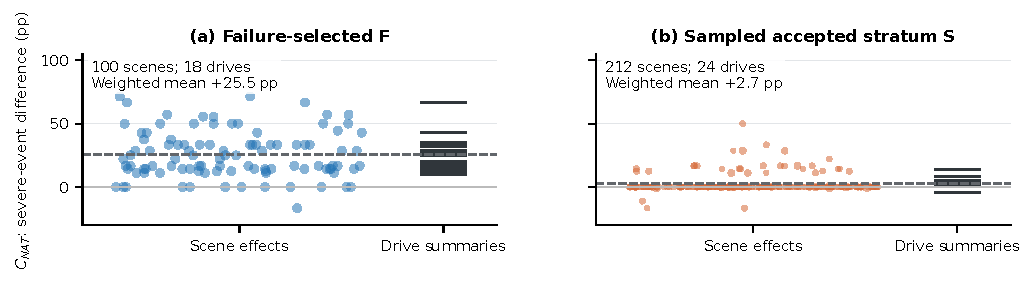
\includegraphics[width=0.95\textwidth]{figS_heterogeneity.pdf}
\caption{\textbf{Scene and drive heterogeneity behind the matched-prefix mean.} Each dot is one scene's $C_{\NAT}$ severe-event difference; accepted-scene dot area increases with its E4 inclusion weight. Black ticks summarize scenes within a drive, preserving weights; dashed lines are stratum means (F: $+25.5$\,pp, 100 scenes/18 drives; S: $+2.7$\,pp, 212 scenes/24 drives). Drive ticks share days/vehicles and are descriptive, not additional independent tests.}
\label{fig:hetero}
\end{figure}

\paragraph{Correction width is not correction duration.} Recent-GT corrects one position at a time. The retained-window run (internally R9) instead holds positions $t^*{+}1,\dots,t^*{+}w$ at GT in every subsequent context (Figure~\ref{fig:width}; same 365 units, 52 development-F scenes, 13 drives). Width three lowers severe events from 45.1\% to 7.6\%, compared with 3.4\% for Full-GT. This recovers 90.1\% (raw 90.05\%) of that run's full-history correction effect, with a descriptive ratio-bootstrap interval $[81.2,98.9]$\%. Units average 2.96 supplied GT positions and 1.90 actual changes. Width eight equals Full-GT for all units because of the ten-token horizon, so late saturation partly reflects exhausted positions.

A transient-exposure check on the earlier start-position set (internally P1-B: 326 failure units with $t^*\leq2$, 46 scenes, 12 drives) recovers 78.3\% $[64.0,86.6]$ with transient GT and 89.0\% $[79.5,98.0]$ with persistent GT (drive bootstrap). It uses a different schedule and does not isolate retention. Neither analysis establishes GT-free recovery after release.

\begin{figure}[h]
\centering
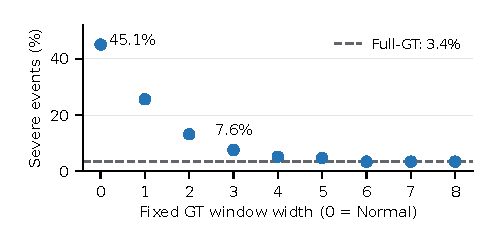
\includegraphics[width=0.45\textwidth]{figS_width.pdf}
\caption{\textbf{Retained GT width, not GT release.} Severe-event rates of the retained-window run (R9) on the same 365 units, 52 scenes, and 13 drives. Points are discrete observed widths, and GT remains in later contexts. Large widths increasingly equal Full-GT because the plan ends. No interval is drawn; this run is distinct from repeated RN/RV.}
\label{fig:width}
\end{figure}

\paragraph{Unit counts 364 vs.\ 365.} No unit was dropped. The 364 motion-response units (one admissible GT-free perturbation per scene and direction sector, up to eight per scene) and the 365 repeated-correction units (the natural forced token plus alternative forced tokens, 52 + 313) are different perturbation families on the same 52 development-F scenes; their unit identifiers do not overlap.

\section{AutoVLA: Additional Measures and Checks}
\label{sec:autovla_more}
\begin{table}[h]
\centering\small
\caption{\textbf{Motion-response endpoint excess at 5\,s} (m; original computation setting). Intervals are approximate drive-cluster percentile bootstraps (10,000 resamples; unit $\to$ scene mean $\to$ drive) with drive-cluster $t$ intervals in parentheses; their coverage was not simulated for this continuous outcome. $p$ is the raw exact drive sign-flip value.}
\label{tab:motionci}
\begin{tabular}{@{}llrrrr@{}}\toprule
Sample & Control & Excess & 95\% interval & Raw $p$ & Units / scenes / drives\\\midrule
F & coordinate accumulation & $+4.37$ & $[3.35,5.20]$ ($[3.35,5.39]$) & 0.00024 & 364 / 52 / 13\\
F & constant motion (CM) & $+2.35$ & $[1.26,3.18]$ ($[1.28,3.42]$) & 0.00073 & 364 / 52 / 13\\
F & learned extrapolator & $+1.97$ & $[1.10,2.83]$ ($[1.07,2.86]$) & 0.0044 & 364 / 52 / 13\\
Selected set & CM & $+0.20$ & $[-0.33,0.55]$ ($[-0.30,0.69]$) & 0.505 & 1,453 / 208 / 19\\
Selected set & learned extrapolator & $-0.34$ & $[-0.78,-0.01]$ ($[-0.73,0.05]$) & 0.074 & 1,453 / 208 / 19\\\bottomrule
\end{tabular}
\end{table}

\begin{table}[h]
\centering\small
\caption{\textbf{NAVSIM v1 non-reactive PDMS of stored plans.} Official scorer through an in-memory metric-cache adapter, 4\,s PDMS horizon; FDE in the severe event uses 5\,s. Approximate cluster-robust $t$ intervals with drive clusters (same policy as the severe-event intervals; E/E4 new-drive coverage not validated). Higher PDMS is better. EPDMS (NAVSIM v2) and two-stage navhard EPDMS were not run on these interventions (they would require new inference); existing navhard EPDMS results on this server concern best-of-$N$ selection rules, not interventions.}
\label{tab:pdms}
\begin{tabular}{@{}llrrrr@{}}\toprule
Contrast & Population & $\Delta$PDMS & 95\% interval & Scenes & Drives\\\midrule
RN & F & $+0.072$ & $[0.034,0.111]$ & 105 & 18\\
RN & E (H\'ajek) & $+0.023$ & $[-0.004,0.049]$ & 353 & 24\\
$C_{\GT}$ & F & $-0.052$ & $[-0.077,-0.027]$ & 100 & 18\\
$C_{\GT}$ & E4 (H\'ajek) & $-0.031$ & $[-0.061,-0.001]$ & 312 & 24\\
$C_{\NAT}$ & F & $-0.055$ & $[-0.093,-0.017]$ & 100 & 18\\
$C_{\NAT}$ & E4 (H\'ajek) & $-0.026$ & $[-0.046,-0.007]$ & 312 & 24\\\bottomrule
\end{tabular}
\end{table}

\paragraph{What the severe event reduces.} Its components move together (Table~\ref{tab:decomp}). For RN in development F, FDE$_{5s}$ falls by 4.06\,m, rule failures by 45.0\,pp, and severe events by 42.8/39.8/36.2/34.6\,pp at FDE thresholds $\tau=2/3/4/5$\,m. The matched-prefix contrasts behave correspondingly with the opposite sign.

\begin{table}[h]
\centering\small
\caption{\textbf{Metric decomposition} (pp unless m). Severe$_\tau$ uses FDE threshold $\tau$\,m; $\tau=3$ is the primary event.}
\label{tab:decomp}
\setlength{\tabcolsep}{3.5pt}
\begin{tabular}{@{}llrrrrrrrr@{}}\toprule
Contrast & Population & FDE$_5$ (m) & ADE$_5$ (m) & Rule fail & Lon.\ fail & Lat.\ fail & Severe$_2$ & Severe$_3$ & Severe$_5$\\\midrule
RN & development F & $-4.06$ & $-1.32$ & $-45.0$ & $-36.7$ & $-14.7$ & $-42.8$ & $-39.8$ & $-34.6$\\
RN & P1-C F & $-3.11$ & $-1.04$ & $-40.6$ & $-34.6$ & $-11.3$ & $-38.4$ & $-34.2$ & $-22.9$\\
RN & P1-C E & $-1.16$ & $-0.40$ & $-4.9$ & $-3.6$ & $-1.8$ & $-4.6$ & $-4.1$ & $-3.2$\\
$C_{\GT}$ & matched F & $+2.41$ & $+0.79$ & $+25.8$ & $+22.8$ & $+7.1$ & $+25.7$ & $+25.3$ & $+18.5$\\
$C_{\NAT}$ & matched F & $+2.35$ & $+0.78$ & $+26.6$ & $+23.1$ & $+7.5$ & $+26.0$ & $+25.5$ & $+18.8$\\
$C_{\NAT}$ & E4 & $+0.91$ & $+0.32$ & $+2.8$ & $+1.9$ & $+1.4$ & $+2.6$ & $+4.0$ & $+3.3$\\\bottomrule
\end{tabular}
\end{table}

\paragraph{Direct-action scope.} Development natural evaluation: 2,748 plans; 1 took the adaptive-reasoning branch and was excluded, leaving 2,747. P1-C stage 1: 5,671 natural plans, 0 generation errors, 0 reasoning-branch stubs, and 0 runaway outputs (more than ten action tokens). Further exclusions were 3,268 plans with no first mismatch to GT tokens and 212 with $t^*>7$, leaving 2,191 eligible (105 F, 2,086 S). Of these, 353 were sampled for intervention, and E4 ($t^*\leq4$) has 1,775 eligible scenes, of which 312 were sampled (100 F, 212 S).

\paragraph{Parity checks.} Exact checks (no-op, hook, and token paths: 1,728--4,008 rows each) gave 0 logit difference and 0 flips. Incremental, deep-invalidation, and cached-versus-recompute paths (480--780 rows each) differed by at most 0.625 logits in bf16. Their 11--105 token flips all met the pre-fixed rule: flips are explained iff $|\Delta\text{logit}|$ and the top-2 margin are within twice the maximum teacher-forced difference. The matched-prefix gate preceded its main run; the repeated-path gate was judged on 2026-10-14, after those runs.

\section{VLA-0 Within-Call Pilot: Implementation}
\label{sec:vla0impl}
\paragraph{Checkpoint and code.} NVlabs VLA-0 code at commit b78db19 and the released LIBERO checkpoint (Hugging Face revision 6c62a51, \texttt{model\_last}; shard hashes recorded) were used without modification. The policy is built on Qwen2.5-VL-3B~\cite{bai2025qwen25vl} and inherits generation settings including repetition penalty 1.05. Prompts, image preprocessing, the digits/space/EOS logits processor, and the action parser are the official ones. The adapter only avoids re-downloading the base model.

\paragraph{Arms and donors.} Within each call, the reference R forces back the natural first three vectors. Arms O, L, and OL replace vector 2, vector 3, or both; secondary arms H and HL also replace vector 1. Donors come from four samples at $T=0.7$ seeded by the observation ID; the first candidate whose vector differs and whose replacement keeps token length and outside-span tokens is used. Edited prefixes enter through forced incremental decoding, which is the native KV path. A first validation attempt that fed prefixes by prefill concatenation failed self-patch identity (3/12); the cause was not established, and the forced-decoding run passed 12/12.

\paragraph{Analyses.} Responses use exactly 35 continuation integers plus EOS for every arm; 149 of 150 pilot observations qualify. For the matched-distance subset, $d_L/d_O$ must lie in $[0.8,1.25]$, where $d_L,d_O$ are mean absolute donor changes over the six arm coordinates in normalized bins. This is a tolerance band, not exact equality. The token-set subset (post hoc) requires R, O, and L prefixes to have the same token set, so the repetition penalty acts on the same tokens; other processor effects are not excluded. In one of 149 observations OL and L produce identical continuations. The direct distance is $D(OL,L)$, whereas $A_{OL}$ and $A_L$ are scalar distances to R. The signed interaction is $J=(30\cdot1000)^{-1}\sum_{\tau=4}^{8}\sum_{d=1}^{6}(s_{OL,\tau d}-s_{L,\tau d}-s_{O,\tau d}+s_{R,\tau d})$; averaging signed coordinates can conceal changes.

\section{VLA-0 Paired Rollouts: Implementation and Full Traces}
\label{sec:vla0cl}
\paragraph{Execution path.} The official LIBERO loop (\texttt{eval\_run}, environment construction, and task loading from the pinned code) runs verbatim, byte-checked against the release tarball. The configuration is that of the README evaluation command: action horizon 1, eight-chunk ensemble version 1, frame skip 10, seed 7, $256\times256$ cameras. The official \texttt{libero\_to\_rv\_obs} conversion requires an uninstalled dependency (lerobot). It is replaced by passing the raw simulator images to the same adapter preprocessing that the pilot validated. The 16/16 smoke-test equality is therefore between the native forward pass and the adapter decoding \emph{for the same actor and preprocessing}; it is not an end-to-end equality through the official conversion function. Executed chunks come from the official text-to-action parser in float32, unchanged into the loop. A logging hook reads the loop's ensemble buffer without modifying it.

\paragraph{Arms, coverage, and checks.} From call 8, L and O apply the donor rule at every call with source seeds fixed by unit and call, so identical inputs receive identical source banks. The two NOT\_APPLIED calls (U1 call 35 and U4 call 22, no eligible donor) executed the natural chunk and are not counted as interventions. The no-op compares R with N bitwise in actions, MuJoCo states, EE poses, and buffers. The offline replay feeds every arm's logged chunks in order, with no stationarity assumption. Simulator determinism replays N's actions in a fresh environment without the model.

\paragraph{Cost and hardware.} The model process held the RTX 5090 for 74.0 wall-clock minutes, including model loading, the smoke test, all 16 paired episodes, and the CPU replays. Peak allocated model memory, from \texttt{torch.cuda.max\_memory\_allocated}, was 8.36\,GB. A post-hoc EGL check under the recorded settings returned Mesa's llvmpipe software renderer; the runtime renderer string was not logged. Only the Mesa EGL vendor was exposed in those settings. Mean times per generation were 2.53\,s natural, 2.79\,s source sampling (4 returns), and 2.50\,s forced decoding.

\begin{figure}[h]
\centering
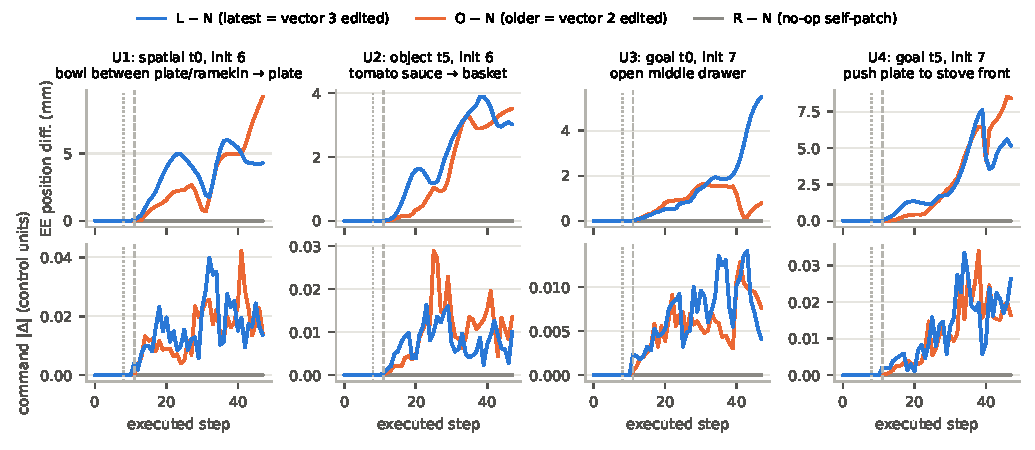
\includegraphics[width=0.95\textwidth]{vla0_closed_loop_supp.pdf}
\caption{\textbf{VLA-0 paired rollouts, full traces.} Top: EE position difference from N (mm). Bottom: mean absolute executed-command difference over the six arm dimensions, in the policy's control units (not meters). Dotted: first edited call (step 8); dashed: first command difference (step 11). All four units and both edits are shown.}
\label{fig:vla0supp}
\end{figure}

\paragraph{Path check without feedback.} Before the rollouts, the official loop was replayed on CPU with stored pilot chunks injected at one call, while all other calls repeated the same chunk. Under the README configuration, context-only edits entered executed offsets 3--7 with weight exactly 1/9 and never offsets 0--2. This stationary replay checks the path only; the closed-loop rollouts measure the actual feedback.

\section{SpatialVLA: Paired Success Counts and Example Paths}
\label{sec:spatial_more}
\begin{table}[h]
\centering\small
\caption{\textbf{SpatialVLA task-level success} (successes out of 120 paired units; $n_{10}/n_{01}$ discordant pairs). Coke uses 120 physical-state clusters (design effect 1); move\_near uses a Rao--Scott design effect for its 10 layouts. Per-task equivalence is not claimed.}
\label{tab:spatialcounts}
\begin{tabular}{@{}lllrrrrr@{}}\toprule
Task & Setting & Contrast & Intervention & Reference & $\Delta$ (pp) & $n_{10}/n_{01}$ & 95\% interval\\\midrule
coke & r1e4 & $R-N$ & 98 & 98 & 0.0 & 7/7 & $[-6.5,6.5]$\\
move\_near & r1e4 & $R-N$ & 94 & 92 & $+1.7$ & 10/8 & $[-8.4,11.7]$\\
coke & r1e4 & $C-F$ & 99 & 94 & $+4.2$ & 11/6 & $[-2.8,11.3]$\\
move\_near & r1e4 & $C-F$ & 95 & 94 & $+0.8$ & 11/10 & $[-6.9,8.6]$\\
coke & r4e1 & $R-N$ & 93 & 91 & $+1.7$ & 19/17 & $[-8.3,11.6]$\\
move\_near & r4e1 & $R-N$ & 85 & 84 & $+0.8$ & 16/15 & $[-8.4,10.0]$\\
coke & r4e1 & $C-F$ & 70 & 75 & $-4.2$ & 16/21 & $[-14.0,5.8]$\\
move\_near & r4e1 & $C-F$ & 77 & 72 & $+4.2$ & 18/13 & $[-8.6,16.7]$\\\bottomrule
\end{tabular}
\end{table}

\begin{figure}[h]
\centering
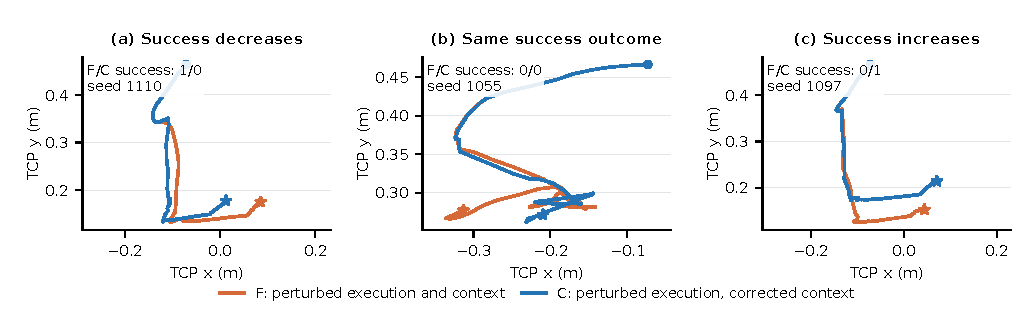
\includegraphics[width=0.95\textwidth]{figS_tcp_paths.pdf}
\caption{\textbf{Actual TCP paths with different paired success outcomes} (r4e1 $C-F$). Examples are selected near the TCP-area median within each post-hoc success-change group, pooling all 240 r4e1 $C-F$ units of both tasks; all three selected cases are move\_near (seeds 1110, 1055, 1097). In groups of even size the two middle units tie, and floating-point rounding decided the pick. Paths are measured in the simulator world frame, with starts marked by dots and ends by stars. Axes differ across cases. Both arms execute the perturbation; C restores reference context, so later actions can differ. The cases are conditioned on the outcome and are not representative samples or causal subgroups. RGB observations were not stored.}
\label{fig:tcp}
\end{figure}

\section{Reproducibility}
\label{sec:repro}
The accompanying archive contains the original author project, the revision tables and provenance records, and the following raw VLA-0 packages in \texttt{raw\_packages/}:
\begin{itemize}
\item the AutoVLA evidence tables (with source paths and hashes);
\item the VLA-0 manifests (validation 12, pilot 150, closed-loop units), the run fingerprints, and the per-call logs (token IDs, prefixes, sources, decoded chunks, input hashes, and dtypes);
\item per-step buffers, actions, MuJoCo states, and EE traces;
\item the analysis, figure, and table-generation scripts used for every number in this revision.
\end{itemize}
Model weights are not included. The VLA-0 runner fixes made after the pilot (fail-fast fingerprinting and a strict validation gate) are for future runs; the completed pilot was produced by the earlier runner, which recorded no runtime fingerprint.

% Original visual-evidence Section I is preserved as Section O.
\section{Visual and Time-Resolved Evidence}
\label{app:visual}
The visual-evidence package adds no model inference or independent experiment. All figures are post-hoc analyses of stored outputs. The complete original package is identified by its SHA-256 in the source provenance record; the paper source contains compact plotting inputs, original selected front-camera images, case arrays, interval policies, and plotting scripts.

\subsection{Case selection and source verification}
The primary candidate set is B2 F at $a=t^*+3$ with one older position: 711 valid paired units in 100 scenes and 18 drives. All units have an available current front-camera image; the image filenames occur in the stored inference keep lists. The shipped raw JPEG bytes have not been verified against the exact preprocessed tensors supplied to the model. Only the current front view is used here; the policy input uses multi-view history. No camera projection or synthetic future image is introduced.

Groups use the sign of the scene-mean severe-event change, NAT\_REF minus NAT\_NSRC: 87 improve, 12 are equal, and one worsens. Equality is of the scene-average binary outcome; individual units or continuous FDE can still differ. Within each group, scenes are ranked by distance to the group-median scene FDE difference, with stable ID ties and a different-drive preference for a second case. Units are selected near the median FDE difference among units whose severe-event change has the group's sign, if any. Thus, scene and displayed-unit differences need not coincide. The rule was fixed before ranking/images in this round, after earlier results were known; it is not preregistration or representative sampling.

\begin{table}[ht]
\centering\small
\caption{All five supplied driving cases. Differences are GT-latest minus Normal-source-latest. $Y$ pairs are GT-latest/Normal-latest. Cases 1 in each group appear in the main figure; the two additional cases are shown below.}
\label{tab:cases}
\begin{tabular}{@{}lrrl@{}}\toprule
Case & Scene-mean FDE change (m) & Displayed-unit FDE change (m) & Displayed $Y$ pair\\\midrule
Improved 1 & $-1.89$ & $-4.96$ & 0/1\\
Improved 2 & $-1.93$ & $-0.50$ & 0/1\\
Unchanged severe rate 1 & $-0.47$ & $-0.37$ & 0/0\\
Unchanged severe rate 2 & $-0.49$ & $-0.67$ & 0/0\\
Worsened 1 & $+2.58$ & $+12.79$ & 1/0\\\bottomrule
\end{tabular}
\end{table}

All 2,160 B2 pairs pass stored token-prefix/hash/pose-prefix equality checks. Recomputed FDE differs from rounded stored values by at most $6.9\times10^{-6}$\,m. The unit-level sign-reversed $C_{\NAT}$ contrast matches exactly, and scene aggregation reproduces the earlier effects. These are internal consistency checks, not proof that every input or statistical assumption is correct.

\begin{figure}[ht]
\centering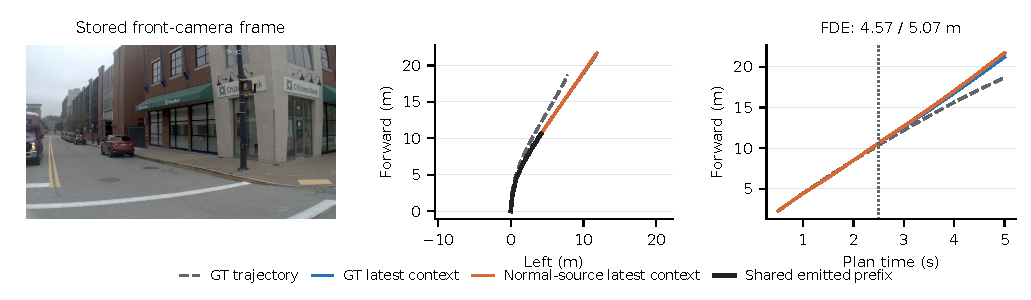
\includegraphics[width=\textwidth]{case_detail_improved_2.pdf}
\caption{Second improved case, from a different drive. Gray is GT, blue GT-latest context, and orange Normal-source-latest context. The emitted black prefix is shared; the vertical line marks the final shared pose time. These are generated plans from one fixed observation.}
\end{figure}
\begin{figure}[ht]
\centering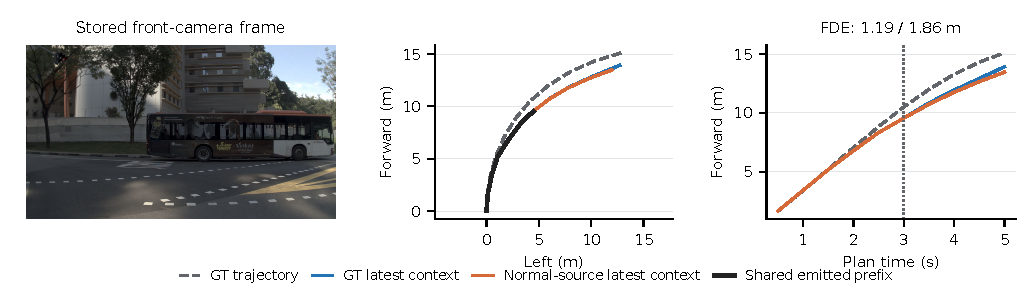
\includegraphics[width=\textwidth]{case_detail_unchanged_severe_2.pdf}
\caption{Second unchanged-severe-rate case. Both displayed plans have $Y=0$, although their trajectories and FDE differ. The image and plan axes are illustrative; camera projection is not inferred.}
\end{figure}
\subsection{Time alignment, fixed support, and accuracy}
The primary time plot uses the same computation-setting-specific unperturbed/perturbed pairs as the endpoint audit. For the fixed common sample, $t_p\leq4$ and relative positions $j=0,\ldots,5$ yield 0--2.5\,s after perturbation at 0.5\,s spacing: 342 F units in 49 scenes, 1,032 accepted units in 147 scenes, and 19 drives overall. These are smaller denominators than the full endpoint sample. All-observable curves in the supplied data have shrinking support (only 17 F scenes at 4.5\,s); they should not be read as fixed-cohort growth curves. No interpolation or new short-horizon severe-event threshold is applied. Curves are descriptive and carry no pointwise or simultaneous coverage claim.

Response size and GT error are computed separately. At 2.5\,s, the common F response is 2.18\,m and CM excess 0.87\,m, while perturbed/unperturbed GT distances are 3.04/3.76\,m. The selected-union GT distances are 1.89/1.73\,m. The sign of a response excess therefore does not identify the sign of an accuracy change.

\begin{figure}[ht]
\centering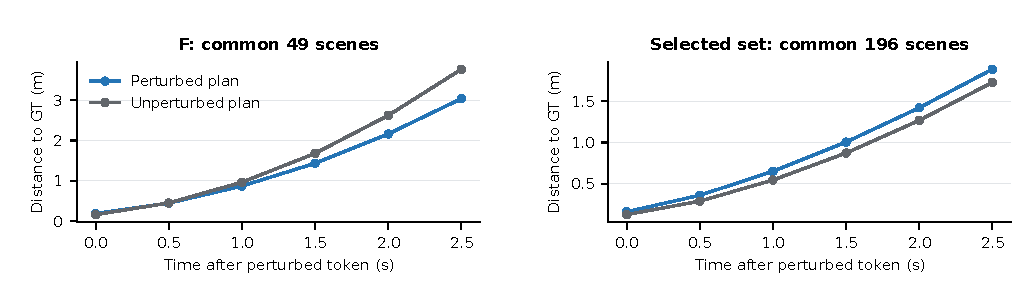
\includegraphics[width=\textwidth]{gt_error_common.pdf}
\caption{GT error on the same fixed common sample used in the main time-response plot. Curves are scene means without inferential bands. F's perturbed plan can be closer to GT despite a larger-than-CM response; the selected union exhibits a different pattern.}
\end{figure}

Unit endpoint distances reproduce the stored motion baseline results to $3.6\times10^{-15}$\,m and aggregate excesses to $8.9\times10^{-16}$\,m. An older deviation-curve file used a batch-one reference; 160/1,453 batch-ten unperturbed plans differ from that reference, with maximum endpoint difference 3.29\,m. Our time and endpoint plots consistently use the same-batch matched reference, as in the existing P2/numerical audit. This pairing distinction changes the descriptive curves, not the frozen endpoint claims. Learned extrapolator traces are endpoint-only; intermediate learned responses are not fabricated.

\begin{figure}[ht]
\centering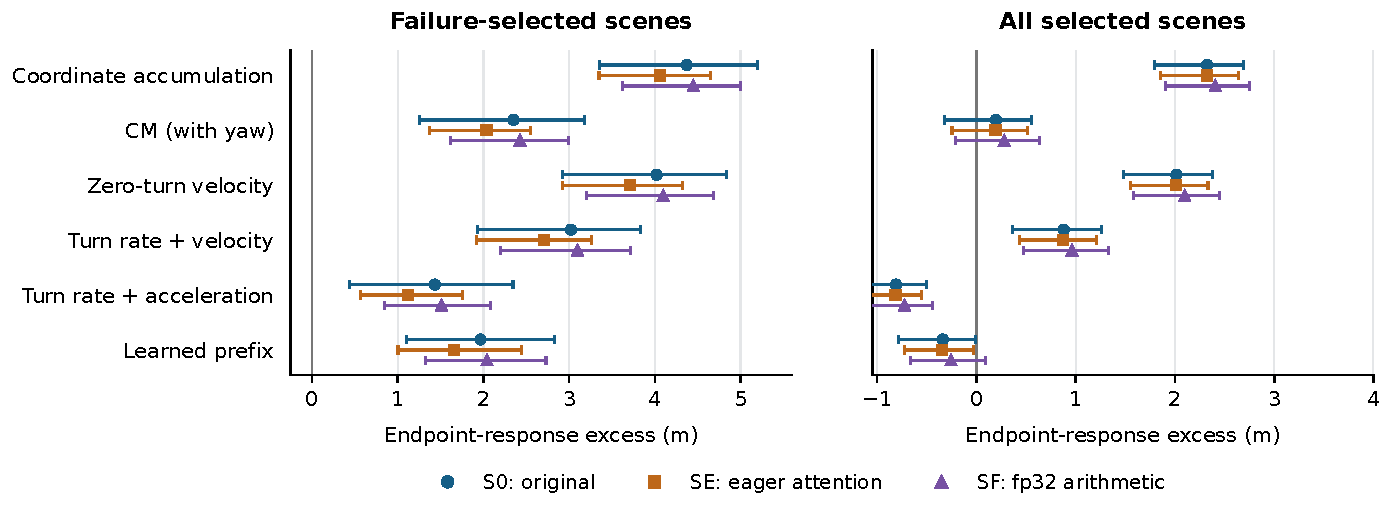
\includegraphics[width=.96\textwidth]{motion_response_20261019.pdf}
\caption{Full endpoint-control comparison retained from the earlier main paper. F and the selected union are distinct cohorts. Bars are descriptive drive-bootstrap intervals with unchecked coverage; the 12 primary tests cover F under SE/SF.}
\end{figure}

\subsection{TCP trajectories and outcome-selected illustrations}
The supplied paired-unit table preserves actual TCP deviations over control steps 0--79. Mean TCP area is 428/449\,cm$\cdot$step for r4e1 $R-N$/$C-F$; the same-success-outcome groups contain 173/172 of the 240 pairs. Large deviations occur in both changed- and unchanged-success groups. Grouping by a post-intervention outcome is descriptive, not a causal subgroup analysis.

\begin{figure}[ht]
\centering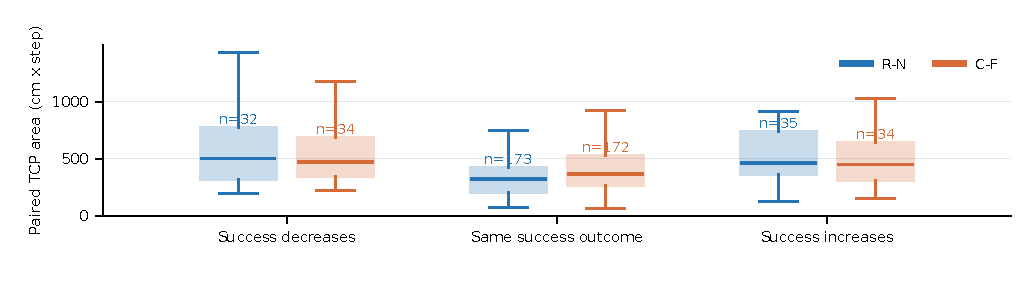
\includegraphics[width=\textwidth]{tcp_area_by_success.pdf}
\caption{r4e1 TCP deviation area by paired success change. Boxes are interquartile ranges with median lines and standard 1.5-IQR whiskers; outliers are not shown. Counts are paired units, not independent physical layouts. Outcome-selected groups describe the recorded episodes and are not used to estimate the pooled success effect.}
\end{figure}

The main TCP cases are the first-ranked $C-F$ case in each success-change group under the supplied median-area rule across both tasks. All three selected examples happen to be \texttt{move\_near}; they do not expand its ten physical layouts. TCP is measured in the simulator world frame (m; stored orientation is quaternion $w,x,y,z$). Only RGB hashes were stored, so no robot photo is presented as an observed frame. Replaying rendered images would be a separate reconstruction, not recovered original observations.

% v03 additions (2026-10-23)
\section{SpatialVLA Within-Call Edits: Path and Discovery Pilot}
\label{sec:svla}
\paragraph{Model and decoding.}
\begin{itemize}
\item \textbf{Model.} We use \texttt{spatialvla-4b-224-sft-fractal} (SigLIP + Gemma~2; transformers 4.47.0; bf16; eager attention) with its official processor and the official SimplerEnv adapter. The adapter uses 224$\times$224 inputs, predicts every control step, ensembles over 4 chunks (temperature $-0.8$) and applies a sticky gripper.
\item \textbf{Output format.} Every natural output in this study has 13 tokens: 4 actions $\times$ (translation, rotation, gripper), then EOS.
\item \textbf{Action coding.} Translation tokens are 4,096 spherical bins and rotation tokens are $16^3$ Euler bins; the gripper takes 2 values.
\item \textbf{Response space.} The official decoder maps tokens to normalized actions before unnormalization. The six motion components of $a_3,a_4$ form the response space. Normalized Euler differences are not geodesic rotations, and these command differences are not end-effector motion.
\item \textbf{Parser.} The official parser zero-pads short outputs and clips out-of-range ids. We therefore check token types ourselves and never pad.
\end{itemize}

\paragraph{Adapter path.}
\begin{itemize}
\item \textbf{Mechanics.} The adapter prefills the prompt once with a HybridCache of length $P{+}256$, as \texttt{generate} does, and then feeds one action token per forward pass. The prompt keeps the official bidirectional mask, and generated or forced tokens are causal. Forced conditioning tokens never enter the prompt.
\item \textbf{Evaluation path.} In the transformers version used, \texttt{generate} stores its cache on the model and reuses it whenever it is long enough. In the discovery pilot, calls made after longer move\_near prompts therefore ran with a larger cache:
  \begin{itemize}
  \item the record-time official output differed from the collection-time output in 7/105 observations;
  \item self-patch identity failed in 4/105 observations.
  \end{itemize}
\item \textbf{Fix and diagnosis.} All reported SpatialVLA results use the official model and processor \emph{with a fresh cache per call}. In a fresh-process diagnostic all affected observations were consistent; deterministic kernels changed tokens and were not used. Three residual first-attempt disagreements were not isolated, and we do not attribute all differences to bf16 arithmetic.
\item \textbf{Logit-level parity.}
  \begin{itemize}
  \item The adapter's natural decoding differs from the official logits by at most 0.125, with no token change.
  \item Self-patch continuation logits are bitwise equal in validation, in the discovery pilot and in the follow-up.
  \item In the drawer task they differ by at most 0.5, again with no token change.
  \end{itemize}
\end{itemize}

\paragraph{Discovery pilot (v01).}
\begin{itemize}
\item \textbf{Path checks.} Self-patch was token-identical in 12/12 validation observations and 105/105 pilot observations (coke: 25 new layouts; move\_near: all 10 layouts, reused).
\item \textbf{Donors.} The first joint-valid donor among four samples was used; 41 observations had none. Of 420 samples, 297 reproduced a natural action.
\item \textbf{Pre-specified primary analysis (distance-matched).} Only 7 observations qualified (6 coke layouts and 1 move\_near layout): $\Delta=0.084$, two-task interval not computed.
\item \textbf{Secondary analysis (all 64 joint-valid observations).} $\Delta=0.070$ $[0.044,0.100]$. On average the L donors were farther than the O donors, so this result is partly confounded by donor distance and is not promoted to a primary result.
\item \textbf{Reselection check.} Among the 420 discovery-pilot samples, any distance-matched candidate existed for only 16 observations in 15 layouts (2 move\_near). This motivated a new, pre-registered donor rule rather than reselection.
\end{itemize}

\section{SpatialVLA Matched Follow-up (v02)}
\label{sec:svla2}
\paragraph{Design (pre-registered before any v02 intervention output).}
\begin{itemize}
\item \textbf{Layouts.} coke uses the first 25 layouts from a survey of seeds 4000--4099 that are disjoint from all discovery-pilot and validation layouts. move\_near reuses the same 10 layouts, seeds and instructions.
\item \textbf{Observations.} Images before natural generation calls 2, 6 and 10 (105 observations). None is identical to a discovery-pilot input.
\item \textbf{Donor rule.} At most 64 sequential official samples per observation ($T{=}0.7$, top-$p$ 1, top-$k$ 0; seeds hashed from the observation id). The first sample that is joint-valid and satisfies $0.8\le d_L/d_O\le1.25$ is used for O, L and OL. If none of the 64 qualifies, the observation is MATCHED\_SOURCE\_MISSING; there is no further search.
\item \textbf{Analysis.} Equal-weight layouts within each task, equal-weight tasks, and a layout bootstrap within tasks (10,000 resamples, seed 20261023).
\item \textbf{Relation to the discovery pilot.} The donor rule and observation calls differ from the discovery pilot, so the two are separate experiments and are never pooled. Because tasks and the move\_near layouts are reused, this is not an independent task-generalization test.
\end{itemize}

\begin{table}[h]
\centering\small
\caption{\textbf{SpatialVLA follow-up denominators} (observations; layouts in parentheses).}
\label{tab:svla2flow}
\begin{tabular}{@{}lrrr@{}}\toprule
Stage & coke & move\_near & Total\\\midrule
Panel layouts & 25 & 10 (reused) & 35\\
Collected observations (calls 2/6/10) & 75 & 30 & 105\\
Valid natural output (12 typed tokens + EOS) & 75 & 30 & 105\\
Path checks pass (official = collection = adapter; R tokens and EOS) & 75 & 30 & 105\\
Matched donor within 64 samples & 55 & 14 & 69\\
Analyzed (valid O/L/OL continuations) & 55 (25) & 14 (9) & 69 (34)\\\bottomrule
\end{tabular}
\end{table}

\paragraph{Sources and coverage.}
\begin{itemize}
\item \textbf{Samples.} 3,243 samples were generated (median 22 per observation). Of these, 2,710 were rejected for zero distance (they reproduced a natural action), 396 for a ratio outside $[0.8,1.25]$ and 68 for a gripper mismatch; 69 were selected.
\item \textbf{Donor distance.} Donor distances are balanced: mean $d_L=0.054$ vs.\ $d_O=0.053$, with ratio quartiles 0.93/1.02/1.16.
\item \textbf{Coverage.} The design target was at least 15 coke and 8 move\_near matched layouts; the run reached 25 and 9.
\item \textbf{Smoke check.} Coke and move\_near observations at call 0 passed all path checks; they are not analyzed.
\end{itemize}

\begin{table}[h]
\centering\small
\caption{\textbf{SpatialVLA follow-up results} (normalized action distance; 95\% layout-bootstrap intervals; 69 observations, 34 layouts).}
\label{tab:svla2res}
\begin{tabular}{@{}lrr@{}}\toprule
Quantity & Estimate & 95\% interval\\\midrule
$\Delta=E_L-E_O$ (primary, two tasks) & 0.048 & $[0.026,0.072]$\\
\ coke (25 layouts) / move\_near (9 layouts) & 0.042 / 0.054 & $[0.015,0.070]$ / $[0.018,0.093]$\\
$E_L$ / $E_O$ & 0.070 / 0.022 & \\
$\Delta$, same change-type pattern at $a_1$ and $a_2$ (48 obs.) & 0.048 & $[0.019,0.079]$\\
$a_3$: $E_L$ / $E_O$; $a_4$: $E_L$ / $E_O$ & 0.068 / 0.027; 0.072 / 0.017 & \\
translation: $E_L$ / $E_O$; rotation: $E_L$ / $E_O$ & 0.076 / 0.020; 0.065 / 0.024 & \\
$D(OL,L)$ (direct) & 0.021 & $[0.012,0.030]$\\
$J=E_{OL}-E_O-E_L$ (descriptive) & $-0.024$ & $[-0.040,-0.011]$\\
gripper change rate in $a_3,a_4$: L / O / OL & 0.082 / 0.053 / 0.067 & \\\bottomrule
\end{tabular}
\end{table}

\paragraph{Reading the follow-up results.}
\begin{itemize}
\item \textbf{Change rates.} The latest edit changed the continuation tokens in 56/69 observations, the older edit in 27/69. In 11 of the 69 observations, $\Delta<0$.
\item \textbf{Older position.} $D(OL,L)>0$ shows that the older position is not irrelevant.
\item \textbf{Interaction.} $J$ is a descriptive interaction; it is not evidence of additivity or of its absence.
\item \textbf{Scope.} These are command-level responses with the intermediate action fixed. They were not executed, and they are not success effects.
\end{itemize}

\begin{figure}[h]
\centering
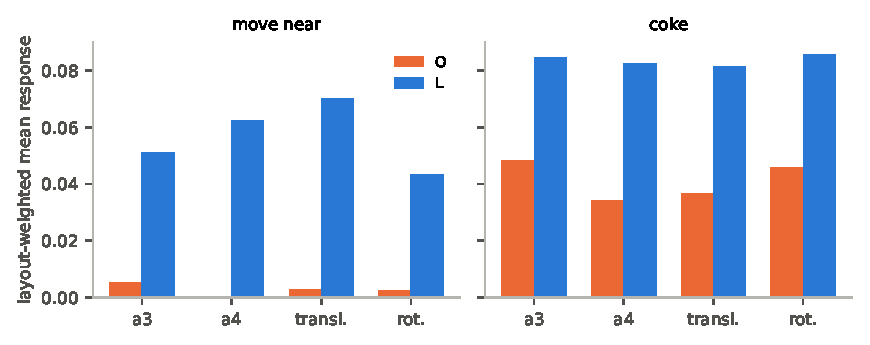
\includegraphics[width=0.75\textwidth]{fig_svla_v02_components.pdf}\\
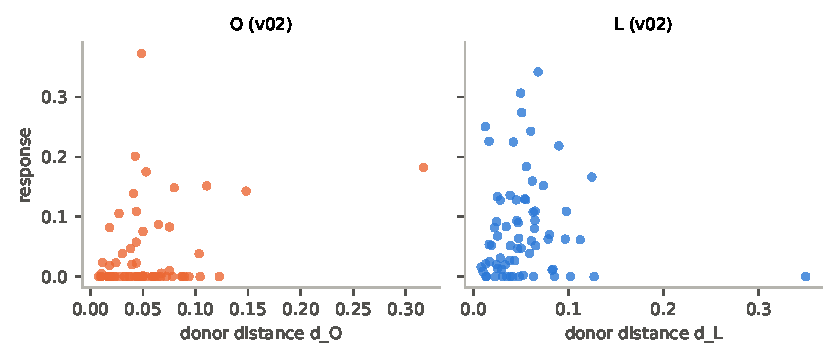
\includegraphics[width=0.6\textwidth]{fig_svla_v02_donor_distance.pdf}
\caption{\textbf{SpatialVLA follow-up: responses by continuation step and component (top) and against donor distance (bottom).} Layout-weighted means; normalized action units.}
\label{fig:svla2comp}
\end{figure}

\section{Supplementary SpatialVLA Task: Open Drawer}
\label{sec:svladrawer}
\paragraph{Task selection.}
\begin{itemize}
\item \textbf{Order checked.} Open drawer, then close drawer.
\item \textbf{Selected task.} \texttt{google\_robot\_open\_drawer} (\texttt{OpenDrawerCustomInScene-v0}).
\item \textbf{Why compatible.} It uses the same Google-robot embodiment, camera path, adapter, checkpoint and normalization, and needs no training. Selection did not use success rates or effects.
\end{itemize}

\paragraph{Panel.}
\begin{itemize}
\item \textbf{Layouts.} The cabinet is fixed; the robot pose and the target drawer vary. A layout is identified by robot and articulation poses plus the instruction. The panel was fixed as the first 20 unique layouts in seeds 5000--5099 (69 unique in total), with calls 2/6/10.
\item \textbf{Collection.} Software rendering of this scene takes about 2.2\,s per step. The first attempt was still collecting after 20.8 GPU-minutes when the process ended: it had collected 44 observations from 16 layouts and produced no intervention outputs.
\item \textbf{Amendment.} An amendment made before any intervention output reused these 44 observations as lossless images. The collection-time output check is therefore unavailable for them; all other path checks ran.
\end{itemize}

\paragraph{Results.}
\begin{itemize}
\item \textbf{Path checks.} Self-patch tokens and EOS were identical in 44/44 observations, and adapter parity held in 44/44.
\item \textbf{Donors.} A matched donor was found within 64 samples for 35/44 observations (15 layouts). Of 1,053 samples, 792 were rejected for zero distance and 226 for the ratio.
\item \textbf{Effect.} $\Delta=0.145$ $[0.091,0.210]$, with $E_L=0.183$ and $E_O=0.039$. Donor distances are balanced (0.100 vs.\ 0.101). $D(OL,L)=0.043$ $[0.020,0.067]$ and $J=-0.057$ $[-0.089,-0.030]$ (descriptive).
\item \textbf{Scope.} This is a single task with a layout-conditional interval, and it is not pooled with the two-task estimand.
\end{itemize}

\begin{figure}[h]
\centering
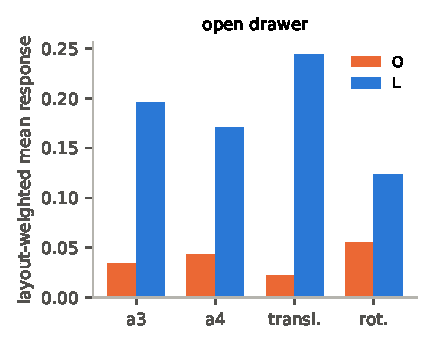
\includegraphics[width=0.45\textwidth]{fig_svla_drawer_components.pdf}\hfill
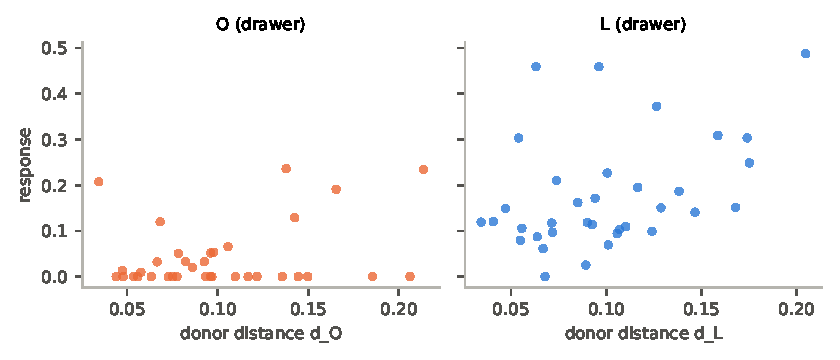
\includegraphics[width=0.52\textwidth]{fig_svla_drawer_donor_distance.pdf}
\caption{\textbf{Open-drawer supplementary task:} responses by step and component (left) and against donor distance (right).}
\label{fig:svladrawer}
\end{figure}

\section{Interventions Compared Across Policies}
\label{sec:crossmodel}
Table~\ref{tab:crossmodel} lists, for each policy, what is edited, what is held fixed, where the response is read, and what the independent unit is. The three within-call contrasts are \emph{not} one shared test.
\begin{itemize}
\item AutoVLA's matched-prefix contrast $C_{\NAT}$ compares a GT and a frozen Normal-source value at the latest position, behind a natural older value, on a binary trajectory event.
\item The VLA-0 and SpatialVLA contrasts directly compare a latest-position edit with an older-position edit, using the same donor on a continuous action distance.
\end{itemize}
In VLA-0 and SpatialVLA, an older-position edit keeps the intermediate action at its natural value. The measured response is therefore a position-specific context response with the intermediate action fixed; it is not total error propagation through the chunk.

\begin{table}[h]
\centering\footnotesize
\caption{\textbf{Within-call interventions by policy.}}
\label{tab:crossmodel}
\setlength{\tabcolsep}{3pt}
\begin{tabularx}{\textwidth}{@{}>{\raggedright\arraybackslash}p{2.3cm} >{\raggedright\arraybackslash}X >{\raggedright\arraybackslash}X >{\raggedright\arraybackslash}X@{}}\toprule
 & AutoVLA (matched prefix) & VLA-0 (within-call pilot) & SpatialVLA (within-call v01 / v02 / drawer)\\\midrule
Backbone; actions & Qwen2.5-VL-3B; 10 motion tokens, one per 0.5\,s & Qwen2.5-VL-3B; 8 vectors of 7 integers as text & SigLIP + Gemma~2; 4 actions of 3 spatial tokens\\
Edited position & latest $a{-}1$ (GT vs frozen Normal token), with older $t^*{+}1$ GT or natural & conditioning vector 3 (L) or 2 (O) & conditioning action $a_2$ (L) or $a_1$ (O)\\
Held fixed & emitted Normal-source prefix through $a{-}1$; source banks frozen & emitted natural vectors 1--3; the non-edited vector natural & emitted natural $a_1,a_2$; the non-edited action natural; donor gripper token equal to natural\\
Donor & frozen Normal-source or GT value (value contrast) & whole vector from 4 $T{=}0.7$ samples & whole action from $T{=}0.7$ samples: first joint-valid of 4 (v01); first distance-matched of $\le$64 (v02, drawer)\\
Response window & suffix from anchor $a$ to the 10th token & vectors 4--8, 6 arm dims & actions $a_3,a_4$, 6 normalized motion dims\\
Contrast & $C_{\NAT}$ (severe-event difference) & $A_L-A_O$ & $E_L-E_O$\\
Executed? & no (open-loop plans) & pilot no; separate paired rollouts executed continuation edits & no (command level)\\
Metric & severe event; PDMS & normalized integer-bin distance & normalized action distance (not metres)\\
Independent unit & drive (also day--vehicle, component) & LIBERO task (30) & physical layout within task (2 tasks; drawer separate)\\\bottomrule
\end{tabularx}
\end{table}

\section{Model Selection: Candidate Policies}
\label{sec:models}
A policy can serve the within-call estimand only if, inside one call, it emits several time steps autoregressively, so that later steps condition on the decoder's copy of earlier ones. Table~\ref{tab:models} summarizes official code and model cards (revisions recorded in the package; L = checked locally, P = public source).

\begin{table}[h]
\centering\footnotesize
\caption{\textbf{Candidate policies for the within-call older-vs-latest estimand.} Surveyed policies are not experimental models of this paper.}
\label{tab:models}
\begin{tabularx}{\textwidth}{@{}l >{\raggedright\arraybackslash}p{2.5cm} >{\raggedright\arraybackslash}X >{\raggedright\arraybackslash}p{3.0cm} l@{}}\toprule
Policy & Backbone & Time step $\leftrightarrow$ token position & Native older/latest edit & Use here\\\midrule
AutoVLA & Qwen2.5-VL-3B & 10 motion tokens, one per 0.5\,s & yes & experiment\\
VLA-0 & Qwen2.5-VL-3B & 8 integer vectors as text, one per step & yes & experiment\\
SpatialVLA-4B & SigLIP + Gemma~2 & 4 actions $\times$ 3 spatial tokens & yes (path verified) & experiment\\
pi0-FAST & SigLIP + Gemma-2B (JAX) & DCT + BPE: a token spans frequency coefficients, not a time step [P] & no (different estimand) & surveyed\\
OpenVLA & DINOv2/SigLIP + Llama-2-7B & one step (7 tokens) per call, no action history [L, P] & no & surveyed\\
OpenVLA-OFT & OpenVLA-7B + LoRA & parallel decoding over zero-embedded slots, regression head [P] & no & surveyed\\
WorldVLA (v1 code) & Chameleon-7B & autoregressive blocks; an inference attention mask blocks attention to earlier action blocks [P] & structural null only & surveyed\\\bottomrule
\end{tabularx}
\end{table}

\paragraph{Why SpatialVLA, and the separate implementation reasons.}
\begin{itemize}
\item \textbf{Scientific reason.} SpatialVLA is the available policy outside the Qwen2.5-VL family whose official decoding exposes a time-ordered within-call channel.
\item \textbf{Implementation reasons} (separate from the scientific reason). Its checkpoint and SimplerEnv setup were already installed and verified. The alternatives need 14--25\,GB of new weights and, for some, new frameworks.
\item \textbf{WorldVLA.} It would provide only an architectural null control. The repository named in its paper now redirects to a successor in which the mask is disabled, so the masked version must be pinned to the original code.
\end{itemize}

\section{Figures Moved from the Main Text in v03}
\label{sec:moved_v03}
To keep the main paper at eight pages after adding the SpatialVLA results, three figures moved here; their numbers remain in the main text.

\begin{figure}[h]
\centering
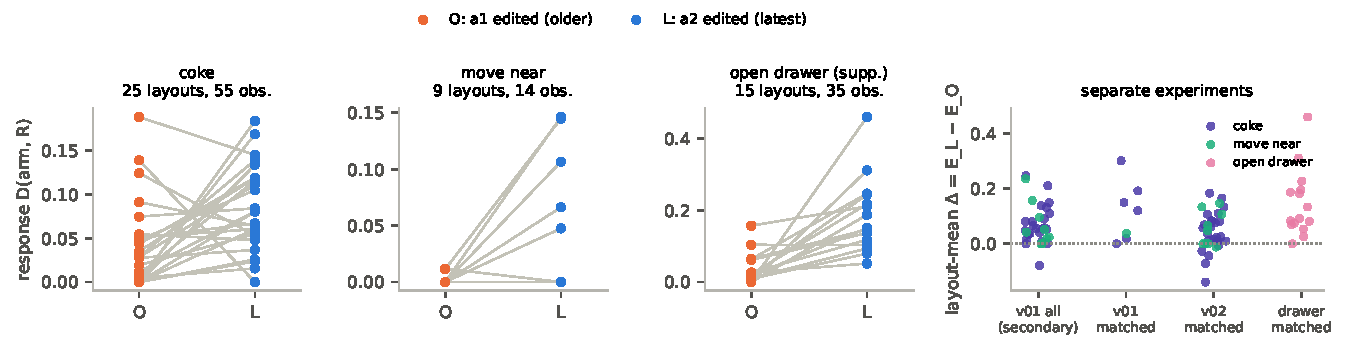
\includegraphics[width=\textwidth]{fig_svla_within_call.pdf}
\caption{\textbf{SpatialVLA within-call responses.} Left three panels: layout-mean responses to the older ($a_1$) and latest ($a_2$) edit in the matched follow-up (coke, move near) and the supplementary open-drawer task. Right: layout-mean $\Delta$ per experiment; experiments use different donor rules or tasks and are not pooled. Normalized action units, not metres.}
\label{fig:svla}
\end{figure}

\begin{figure}[h]
\centering
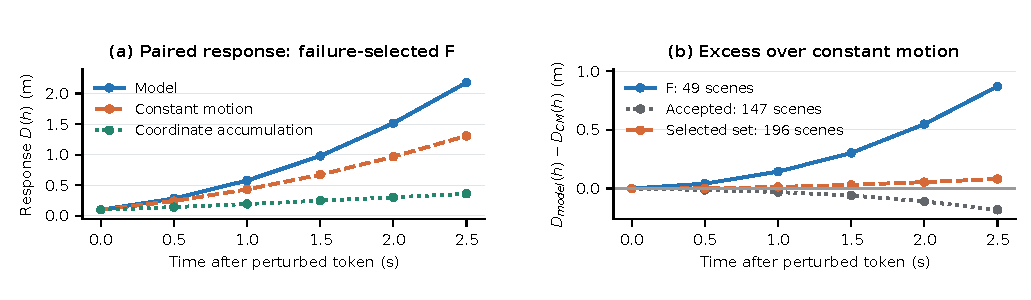
\includegraphics[width=\textwidth]{fig_time_resolved.pdf}
\caption{\textbf{AutoVLA: plan response beyond constant motion is concentrated in failure-selected plans.} Post-hoc curves under the original computation setting on a fixed common sample with perturbation position $t_p\leq4$: F has 342 units/49 scenes/13 drives; accepted has 1,032 units/147 scenes; their selected union has 19 drives. Left: paired response magnitudes in F. Right: excess over CM per stratum and in the union. Curves are scene means without inferential bands. Response magnitude is distinct from GT error.}
\label{fig:time}
\end{figure}

\begin{figure}[h]
\centering
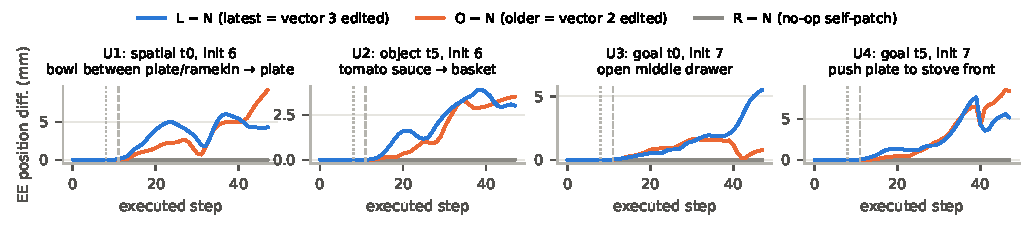
\includegraphics[width=\textwidth]{vla0_closed_loop_main.pdf}
\caption{\textbf{VLA-0: context-only edits change executed motion.} EE position difference (mm) from N after each executed step, for all four units and both edits (U1: spatial task 0, U2: object task 5, U3/U4: goal tasks 0/5; initial states 6/6/7/7). Dotted line: first edited call (step 8); dashed: first executed-command difference (step 11). R$-$N (gray) is zero. Command differences in control units are in Fig.~\ref{fig:vla0supp}.}
\label{fig:vla0cl}
\end{figure}

